\section{问题一：确定性最优调度}

\subsection{能量流与储能状态模型}
附件1给出完整单日的负荷、光伏和电价，故本问不引入预测误差。将全天划分为
$\mathcal T=\{0,1,\ldots,143\}$共144个10分钟区间，$\Delta t=1/6\ \mathrm{h}$。
以$g_t,c_t,d_t,w_t$分别表示外网购电、充电、放电和弃光功率，$E_t$表示区间$t$
起点的储能电量（kWh），而非比例SOC。每一时段满足
\begin{equation}
 g_t+P_t+d_t=L_t+c_t+w_t,
 \label{eq:p1-balance}
\end{equation}
其中$0\le w_t\le P_t$，即弃光只能来自当期光伏。储能状态按实际充、放电效率递推：
\begin{equation}
 E_{t+1}=E_t+\eta_c c_t\Delta t-\frac{d_t\Delta t}{\eta_d}.
 \label{eq:p1-soc}
\end{equation}
题设参数为$\eta_c=\eta_d=0.9$、$P_{\max}=5000\ \mathrm{kW}$，且
$1200\le E_t\le10800\ \mathrm{kWh}$。问题一采用单日闭环条件
$E_0=E_{144}=6000\ \mathrm{kWh}$，以排除通过透支期末电量降低当日费用的方案。

\subsection{确定性储能--购电MILP}
引入二元变量$u_t$表示充电状态；$u_t=1$时允许充电，$u_t=0$时允许放电。
问题一的正式模型为
\begin{equation}
\begin{aligned}
\min\quad &\sum_{t\in\mathcal T}p_tg_t\Delta t\\[-2pt]
\text{s.t.}\quad&
\left\{\begin{aligned}
 g_t+P_t+d_t&=L_t+c_t+w_t,&&t\in\mathcal T,\\
 E_{t+1}&=E_t+\eta_c c_t\Delta t-d_t\Delta t/\eta_d,
     &&t\in\mathcal T,\\
 E_{\min}\le E_t&\le E_{\max},&&t=0,\ldots,144,\\
 0\le c_t&\le P_{\max}u_t,&&t\in\mathcal T,\\
 0\le d_t&\le P_{\max}(1-u_t),&&t\in\mathcal T,\\
 u_t&\in\{0,1\},&&t\in\mathcal T,\\
 g_t&\ge0,\quad 0\le w_t\le P_t,&&t\in\mathcal T,\\
 E_0&=E_{144}=6000.
\end{aligned}\right.
\end{aligned}
\label{eq:p1-model}
\end{equation}
目标函数只计外网购电支出，不含售电收益、充放电补贴、循环奖励或电池退化成本。
二元变量仅用于排除同一10分钟区间内的同时充、放电；正式结果采用CBC求解该MILP。

\subsection{充放电互补约束的条件性精确松弛}
为解释互补约束在本模型中的作用，考虑删除$u_t$并分别保留
$0\le c_t,d_t\le P_{\max}$所得的LP松弛。记$\alpha=\eta_c\eta_d<1$。

\textbf{命题1（可行交换条件下的互补精确松弛）}
若该LP存在一个最优解，使其中每个$c_t>0,d_t>0$的时段均满足
\begin{equation}
 g_t+P_t-w_t\ge
 (1-\alpha)\min\left\{c_t,\frac{d_t}{\alpha}\right\},
 \label{eq:p1-exchange-condition}
\end{equation}
则至少存在一个满足$c_td_t=0$的LP最优解，因而该条件下MILP与LP的最优目标值相同。

\begin{samepage}
\textit{证明概要：}
对任一同时充、放电时段，令
$\delta=\min\{c_t,d_t/\alpha\}$、$r=(1-\alpha)\delta$。
作如下变换：
\begin{equation}
 c'_t=c_t-\delta,\qquad d'_t=d_t-\alpha\delta.
 \label{eq:p1-exchange}
\end{equation}
由于$\alpha/\eta_d=\eta_c$，式\eqref{eq:p1-exchange}保持该时段的储能增量不变，
故全部后续$E_t$及终端条件均不变；同时至少有$c'_t,d'_t$之一为0。该变换在功率平衡中
释放$r$的供给余量。由式\eqref{eq:p1-exchange-condition}，可将其分解为减少购电$a_t$
和增加弃光$b_t$，其中$a_t+b_t=r$、$0\le a_t\le g_t$、
$0\le b_t\le P_t-w_t$。于是功率平衡、变量边界和功率上限仍成立，而目标函数变化为
$-p_ta_t\Delta t\le0$。逐时重复即可得到互斥可行解；再结合LP是MILP的松弛，得到两者
最优值相等。完整交换论证见附录\ref{app:p1-relaxation-proof}。
\end{samepage}

非负电价、无售电收益和无循环补贴保证上述交换不会增加费用；式
\eqref{eq:p1-exchange-condition}则是保持外网非负与弃光上界所需的可行性条件。因此，该命题是
条件性结论，并不声称所有LP可行解或最优解都会自然互斥。

\subsection{LP--MILP数值交叉验证}
对附件1实例，正式MILP与仅删除二元模式变量及两条互斥约束的LP使用完全相同的功率平衡、
储能递推、功率与电量边界、弃光约束和首末电量。表\ref{tab:p1-lp-relaxation}中的数据直接
来自同口径审计结果。
% Source: results/problem1/tables/q1_lp_relaxation_comparison.csv
\begin{table}[H]
\centering\small
\caption{附件1单日算例的MILP与LP松弛同口径对照}
\label{tab:p1-lp-relaxation}
\setlength{\tabcolsep}{7pt}
\begin{tabular}{lrr}
\toprule
指标 & 正式MILP & LP松弛 \\
\midrule
目标值/元 & 35126.948591 & 35126.948591 \\
外网购电量/kWh & 59482.699 & 59482.699 \\
充电量/kWh & 20740.666 & 20740.666 \\
放电量/kWh & 16799.940 & 16799.940 \\
弃光量/kWh & 0 & 0 \\
储能电量范围/kWh & 1200--10800 & 1200--10800 \\
最大同时充放电功率/kW & 0 & 0 \\
同时充放电区间数 & 0 & 0 \\
单次求解用时/s & 0.211 & 0.067 \\
\bottomrule
\end{tabular}
\end{table}

两者目标值均为$35126.948591$元，绝对与相对松弛间隙均为0；LP最大同时充放电功率为0，
求解用时由$0.211$ s降至$0.067$ s，单次计时比约为3.1。两解仅在5个等价时段的功率分配
存在数值差异，其中3个时段的差异超过$10^{-3}$，但全天购电、充电、放电、弃光及SOC边界
完全一致。由此，理论结构解释与数值证书共同表明：LP松弛在附件1这一确定性单日算例上精确，
但该结论不推广至问题二至四的随机、多阶段或滚动模型；正式主模型仍为MILP。

\subsection{效率修正的局部套利判据}
考虑仅由价差驱动的两个理想化时段$i$和$j$。若时段$i$从外网额外购买$1\ \mathrm{kWh}$
用于充电，则进入储能$\eta_c\ \mathrm{kWh}$，未来能够向负荷释放
$\eta_c\eta_d\ \mathrm{kWh}$。忽略功率和电量边界等耦合约束时，正的纯价格套利空间要求
\begin{equation}
 p_j\eta_c\eta_d>p_i,
 \qquad\text{即}\qquad
 \frac{p_j}{p_i}>\frac{1}{\eta_c\eta_d}.
 \label{eq:p1-arbitrage-threshold}
\end{equation}
在$\eta_c=\eta_d=0.9$时，阈值为$1/0.9^2\approx1.235$。这是理想化、局部的效率修正
套利判据，并非全局最优策略的充分必要条件；实际决策还同时受SOC边界、功率上限、光伏出力、
负荷需求和终端SOC约束影响。图\ref{fig:p1-dispatch}显示充电主要位于低价或光伏富余时段，
放电主要位于较高价格时段，实际轨迹与上述经济机制总体一致。

\subsection{求解结果与灵敏度}
无储能对照按$g_t=(L_t-P_t)_+$购电、$w_t=(P_t-L_t)_+$弃光。
表\ref{tab:p1-summary}在相同负荷、光伏和电价下比较经济收益与物理可行性。
正式MILP达到Optimal，购电费用为$35126.948591$元，较无储能对照的$48052.047$元
减少$12925.098$元，节费率为$26.898\%$；外网购电量为$59482.699\ \mathrm{kWh}$，
原有$6247.963\ \mathrm{kWh}$弃光被全部消纳，储能电量始终处于
$1200$--$10800\ \mathrm{kWh}$。
\begin{table}[H]
\centering\small
\caption{问题一经济收益与物理核验}\label{tab:p1-summary}
\setlength{\tabcolsep}{4pt}
\begin{tabular}{lrrl}
\toprule
指标 & 无储能对照 & 正式MILP & 改善或核验 \\
\midrule
购电费用/元 & 48052.047 & 35126.948591 & 节省12925.098 \\
节费率 & -- & -- & 26.898\% \\
外网购电量/kWh & 61789.935 & 59482.699 & 减少2307.236 \\
弃光量/kWh & 6247.963 & 0 & 全部消纳 \\
储能电量/kWh & 不适用 & 1200--10800 & 首末均为6000 \\
最大功率平衡残差/kW & -- & $4.0\times10^{-5}$ & 通过 \\
最大电量递推残差/kWh & -- & $4.7\times10^{-4}$ & 通过 \\
\bottomrule
\end{tabular}
\end{table}


\begin{figure}[htbp]
\centering
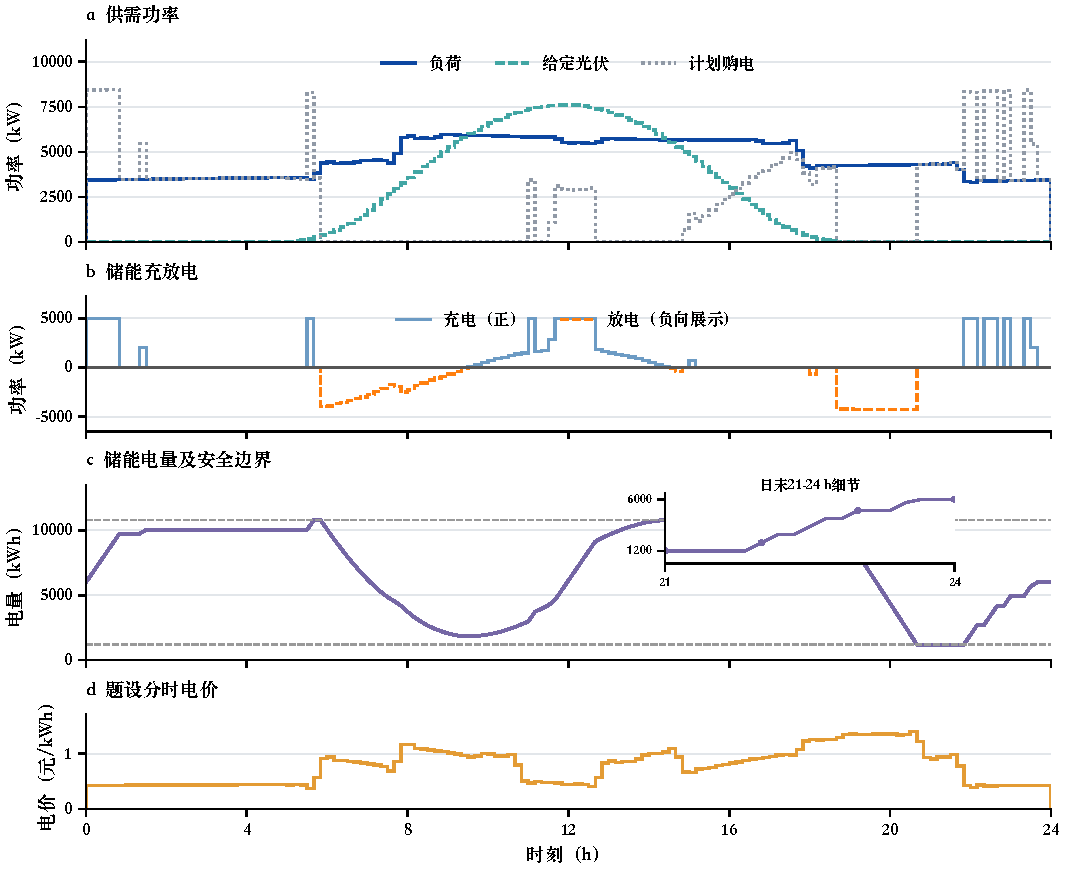
\includegraphics[width=.94\textwidth]{figures/redesign/fig_q1_dispatch.pdf}
\caption{附件1确定性最优轨迹：供需功率、充放电、储能电量与电价。放电以负向展示以区分动作；
虚线为电量边界，嵌图放大21--24时的原轨迹；各曲线均为单次确定性解，无误差带。}
\label{fig:p1-dispatch}
\end{figure}

题目指定区间购电量$q_t=g_t\Delta t$见表\ref{tab:p1-purchase-samples}，
六个4小时区间的充放电量见表\ref{tab:p1-storage-blocks}，所有电量单位均为kWh。
\begin{table}[htbp]
  \centering
  \caption{微网在指定时间段的购电量及全天的购电量和购电费}
  \label{tab:p1-purchase-samples}
  \small
  \begin{tabular}{crcrcr}
    \toprule
    时间段 & 购电量 & 时间段 & 购电量 & 时间段 & 购电量 \\
    \midrule
    10:00--10:10 & 0.000   & 12:00--12:10 & 486.403 & 14:00--14:10 & 0.000 \\
    16:00--16:10 & 394.931 & 18:00--18:10 & 636.983 & 20:00--20:10 & 0.000 \\
    \midrule
    全天购电量 & \multicolumn{2}{c}{59482.699 kWh}
      & 全天购电费 & \multicolumn{2}{c}{35126.949 元} \\
    \bottomrule
  \end{tabular}
\end{table}

全天累计充电$20740.666\ \mathrm{kWh}$，累计放电$16799.940\ \mathrm{kWh}$；
二者差异来自充、放电效率损耗。六个4小时区间的储能吞吐量如下。
\begin{table}[htbp]
  \centering
  \caption{储能设备在指定时间段的充放电量及0:00和24:00的储电量}
  \label{tab:p1-storage-blocks}
  \small
  \begin{tabular}{crrcrr}
    \toprule
    时间段 & 充电量 & 放电量 & 时间段 & 充电量 & 放电量 \\
    \midrule
    0:00--4:00   & 4500.000 & 0.000    & 4:00--8:00   & 833.333  & 6365.841 \\
    8:00--12:00  & 4787.964 & 1702.997 & 12:00--16:00 & 5286.035 & 91.101 \\
    16:00--20:00 & 0.000    & 5780.132 & 20:00--24:00 & 5333.333 & 2859.868 \\
    \midrule
    0:00储电量 & \multicolumn{2}{c}{6000.000 kWh}
      & 24:00储电量 & \multicolumn{2}{c}{6000.000 kWh} \\
    \bottomrule
  \end{tabular}
\end{table}

\newcommand{\QOneEffLowCost}{38223.65}
\newcommand{\QOneEffHighCost}{33767.03}
\newcommand{\QOneEffReduction}{11.66}
\newcommand{\QOneCapacityGainFirst}{2850.82}
\newcommand{\QOneCapacityGainSecond}{2042.64}
\newcommand{\QOneCapacityGainThird}{1570.20}
\newcommand{\QOnePowerGainFirst}{1043.97}
\newcommand{\QOnePowerGainSecond}{219.92}
\newcommand{\QOnePowerGainThird}{53.93}
\newcommand{\QOneEffElasticity}{0.697}
\newcommand{\QOneCapacityElasticity}{0.179}
\newcommand{\QOnePowerElasticity}{0.006}

采用单因素分析，效率取$\eta_c=\eta_d\in\{0.80,0.85,0.90,0.95\}$，容量及功率上限
各取基准的$0.50,0.75,1.00,1.25$倍，其余条件不变；容量变化时，电量下界、上界和
首末值分别保持为容量的10\%、90\%、50\%。12个情形均达到最优并通过物理核验，结果见
图\ref{fig:p1-sensitivity}。
\begin{figure}[htbp]
\centering
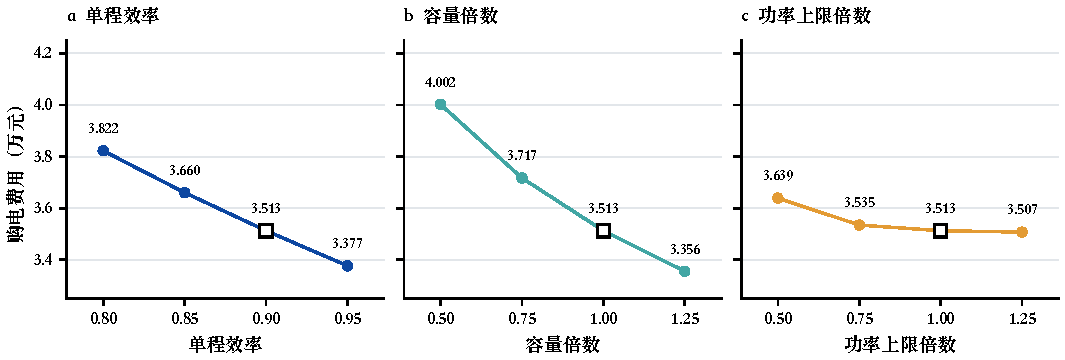
\includegraphics[width=.98\textwidth]{figures/redesign/fig_q1_sensitivity.pdf}
\caption{单因素灵敏度。圆点为已求解的确定性情形，空心方框为基准配置，连线仅辅助比较；
纵轴为明示的局部费用尺度，不设误差棒。}
\label{fig:p1-sensitivity}
\end{figure}
单程效率从0.80增至0.95，费用下降\QOneEffReduction{}\%。容量每增加3000 kWh，
费用依次减少\QOneCapacityGainFirst{}、\QOneCapacityGainSecond{}、
\QOneCapacityGainThird{}元；功率每增加1250 kW，依次减少\QOnePowerGainFirst{}、
\QOnePowerGainSecond{}、\QOnePowerGainThird{}元，均呈边际收益递减。从基准向相邻较高
设定的有限步长归一化敏感度看，效率损耗影响最大、容量次之，5000 kW以上继续增加功率的
收益已很小。该判断限于本日输入和所测参数区间，不等价于投资最优结论。

问题一建立的变量--约束式储能调度骨架将在后续问题中保持不变，并通过增加不确定场景、
多时点结算及动态价格机制逐级扩展。
